\begin{figure*}[!t]
    \centering
    \begin{subfigure}[b]{0.315\textwidth}
        \centering
        \begin{tikzpicture}
            \node[anchor=south west, inner sep=0pt] (img) at (0,0) {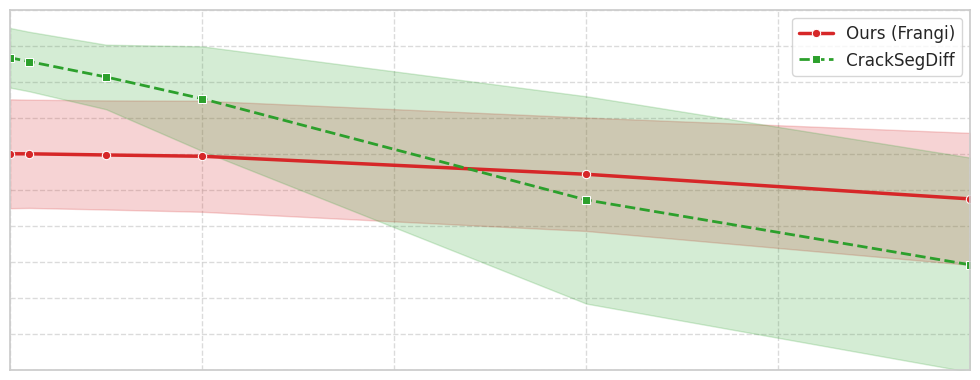
\includegraphics[width=0.84\linewidth]{Jaccard_noisy.png}};
            \useasboundingbox (img.south west) rectangle (img.north east);
            \draw[-latex, thin] (img.south west) -- (img.south east) -- ++(12pt,0) node[above left, inner sep=1pt, font=\scriptsize] {Noise};
            \draw[-latex, thin] (img.south west) -- (img.north west) -- ++(0,12pt) node[above, font=\scriptsize] {Score (\%)};
            \node[below left, font=\scriptsize] at (img.south west) {$0$};
            \node[below, font=\scriptsize] at (img.south east) {$0.5$};
            \node[left, font=\scriptsize] at (img.north west) {$100$};
        \end{tikzpicture}
        \caption{\textsc{Jaccard}}
    \end{subfigure}
    \hfill
    \begin{subfigure}[b]{0.315\textwidth}
        \centering
        \begin{tikzpicture}
            \node[anchor=south west, inner sep=0pt] (img) at (0,0) {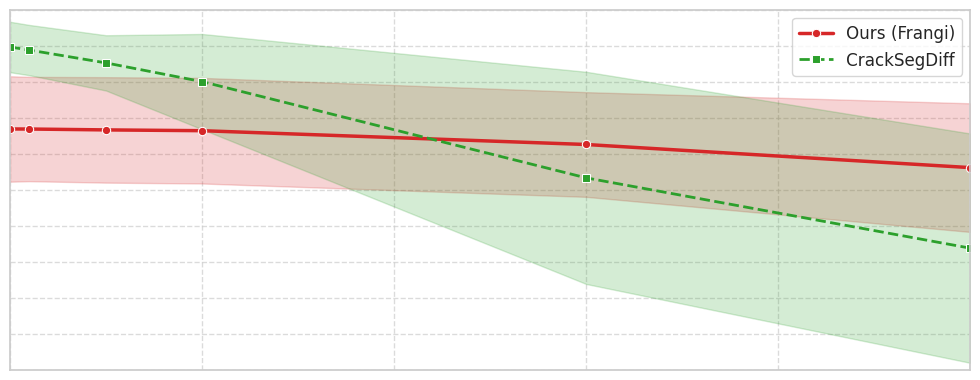
\includegraphics[width=0.84\linewidth]{Tversky_noisy.png}};
            \useasboundingbox (img.south west) rectangle (img.north east);
            \draw[-latex, thin] (img.south west) -- (img.south east) -- ++(12pt,0) node[above left, inner sep=1pt, font=\scriptsize] {Noise};
            \draw[-latex, thin] (img.south west) -- (img.north west) -- ++(0,12pt) node[above, font=\scriptsize] {Score (\%)};
            \node[below left, font=\scriptsize] at (img.south west) {$0$};
            \node[below, font=\scriptsize] at (img.south east) {$0.5$};
            \node[left, font=\scriptsize] at (img.north west) {$100$};
        \end{tikzpicture}
        \caption{\textsc{Tversky}}
    \end{subfigure}
    \hfill
    \begin{subfigure}[b]{0.315\textwidth}
        \centering
        \begin{tikzpicture}
            \node[anchor=south west, inner sep=0pt] (img) at (0,0) {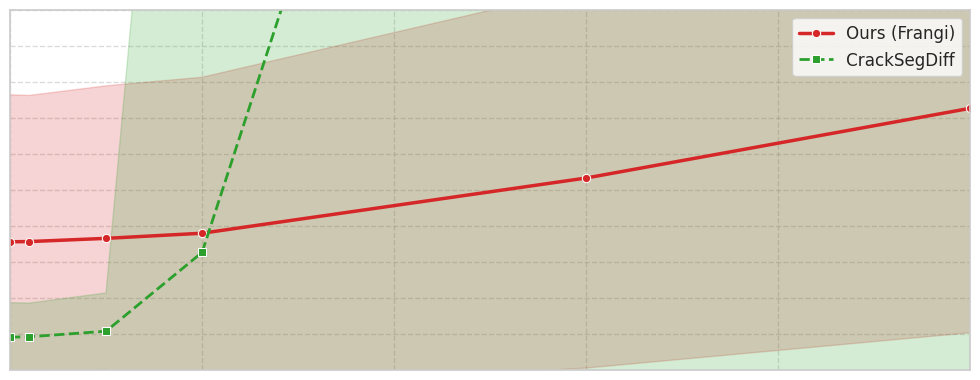
\includegraphics[width=0.84\linewidth]{Wasserstein_noisy.png}};
            \useasboundingbox (img.south west) rectangle (img.north east);
            \draw[-latex, thin] (img.south west) -- (img.south east) -- ++(12pt,0) node[above left, inner sep=1pt, font=\scriptsize] {Noise};
            \draw[-latex, thin] (img.south west) -- (img.north west) -- ++(0,12pt) node[above, font=\scriptsize] {Dist. (px)};
            \node[below left, font=\scriptsize] at (img.south west) {$0$};
            \node[below, font=\scriptsize] at (img.south east) {$0.5$};
            \node[left, font=\scriptsize] at (img.north west) {$100$};
        \end{tikzpicture}
        \caption{\textsc{Wasserstein}}
    \end{subfigure}
    \caption{Performance degradation on noisy FIND. Red: Proposed method; Green: CrackSegDiff. Shaded regions show standard deviation. The horizontal axis is the noise level $s$ (standard deviation of the Gaussians).}
    \label{fig:Results_noisy}
\end{figure*}
